\documentclass[11pt]{article} % do not change this line
\input{BigDataStyle.txt}      % do not change this line
\usepackage{amsmath,amsfonts,amssymb,amsthm,latexsym,graphicx}

\emergencystretch=5mm
\tolerance=400
\allowdisplaybreaks[4]

\graphicspath{ {./images/} }

\theoremstyle{plain}
\newtheorem{theorem}{Theorem}[section]
\newtheorem{proposition}[theorem]{Proposition}
\newtheorem{corollary}[theorem]{Corollary}
\newtheorem{lemma}[theorem]{Lemma}
\newtheorem{problem}[theorem]{Problem}

\theoremstyle{definition}
\newtheorem*{remark}{Remark}

\title{Deep Learning}
\author{Michael Harrison}

\newcommand{\Programme}{Machine Learning}
% Computational Finance students: uncomment the next line
%\twodepartmentstrue

\begin{document}
\maketitle

\declaration

\begin{acknowledgement}
I would like to thank...
\end{acknowledgement}

% NB: The abstract environment also inserts the Table of Contents
\begin{abstract}
ABSTRACT TBD
\end{abstract}


% BEGIN INTRODUCTION
\newpage
\setcounter{page}{1}
\pagenumbering{arabic}
\section{Introduction}
The aim of this project is to explore the use of Deep Learning models in a practical situation. In particular, we have focused on using neural networks to classify x-ray images as normal or abnormal.

% END INTRODUCTION


% BEGIN BACKGROUND
\newpage
\section{Background}
This is the Background section!

\subsection{Convolutional Neural Networks}
Write about conv nets, their performance, history etc

\subsection{Training}
Write about training nets, loss functions, optimisers etc

\subsection{Prediction}
Write about generating predictions from the networks

\subsection{Performance Measures}
Write about performance measures - ROC curve, Cohen's Kappa etc
Discuss train vs valid performance, overfitting etc.

\subsection{State-of-the-Art}
What is the current image processing SOTA - e.g. ILSVRC
Anything done specifically for radiology?

\subsection{Pretrained Models}
Discuss the use of pre-trained models - can keep weights the same, replact the head.
Describe the structure of the pre-trained models we'll use for comparison:
[MAYBE PUT INTO APPENDIX?] 
\subsubsection{VGG16}
Describe VGG16 \\
An example of a reference:
\cite{hastie/etal:2009}.

% END BACKGROUND


% BEGIN DATA
\newpage
\section{Data}
Write about the MURA data, show some exmaple images (normal \& abnormal), give data breakdowns 

\subsection{MURA}
Discuss MURA - what it is, how it was produced

\subsection{Image Examples}
As can be seen in \textbf{Figure \ref{fig:xray1}} below, the x-ray is of a hand. A side-profile of the hand from the same study can be seen in \textbf{Figure \ref{fig:xray2}}. \textbf{Figure \ref{fig:xray2_copy}} is a copy of \textbf{Figure \ref{fig:xray2}}.

\begin{figure}
  \centering    
  \caption{Example X-Ray Image}
  \label{fig:xray1}
  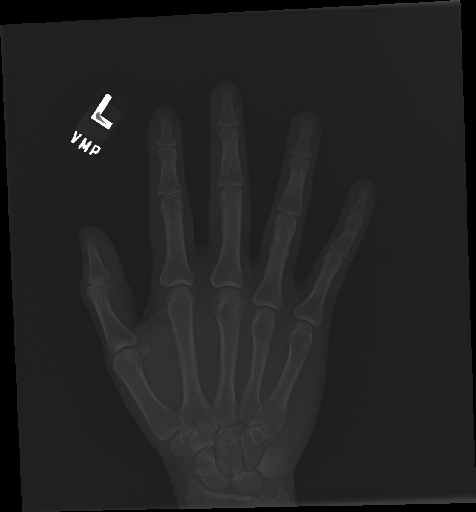
\includegraphics[scale=0.5]{image1.png}
  \caption{Another example X-Ray Image}
  \label{fig:xray2}
  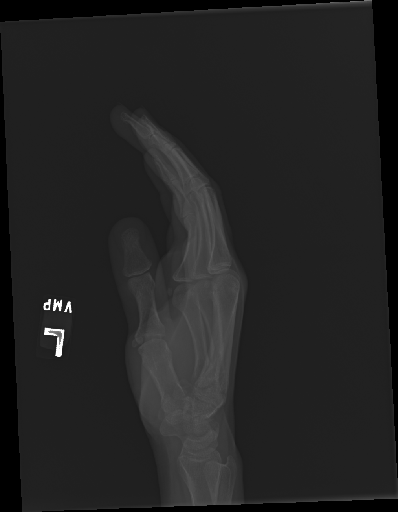
\includegraphics[scale=0.5]{image2.png}
  \caption{A copy of figure 2}
  \label{fig:xray2_copy}
  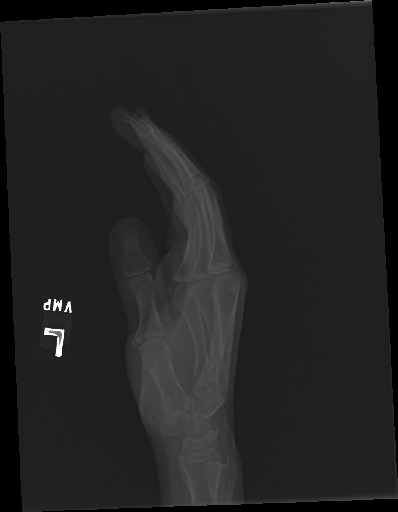
\includegraphics[scale=0.5]{image2_copy.png}
\end{figure}
\clearpage
\noindent

\subsection{Data Breakdowns}
Here's another example of a reference \cite{MURA2017} inline within the text

% END DATA


% BEGIN MODEL DEVELOPMENT
\newpage
\section{Model Development}

\subsection{Working Environment}
Describe google cloud set-up, GPU, python packages used etc

\subsection{Data Preprocessing}
Describe the preprocessing work done on the data - resize images, normalise values, data augmentation etc 

\subsection{Model}
Describe the final ab-initio model I end up with - structure, loss function, training params/hyperparams etc

\subsection{Predictions}
Discuss getting predictions and aggregating down to study-level predctions

% END MODEL DEVELOPMENT


% BEGIN RESULTS
\newpage
\section{Results}

\subsection{Baseline Performance}
Give the performance of my chosen ab-initio model

\subsection{Image Size}
How do my results vary with size of image? Does increasing image size increase scope for

\subsection{Regularisation}
Perform some regularisation experiments, show results

\subsection{Pre-Trained Models}
How does my model compare vs a selection of pretrained models

% END RESULTS


% BEGIN CONCLUSIONS
\newpage
\section{Conclusions}
Include introspective chapter
Work here not comaparable to clinical setting, e.g. smaller, lower resoution images; radiologist may have a relationship with patient - know medical history, other symptoms etc
What is "abnormal"? - type \& severity of abnormality not known, MURA paper not clear.

% END CONCLUSIONS


% BEGIN ETHICAL
\newpage
\section{Professional and Ethical Issues}
Potential Impact on Radiology - Deep Learning tools used to help triage/prioritise radiologists' work, not replace them; 
Can we trust diagnosis to a computer program? Would you be happy to do so? 
Conversely - medical errors happen a lot (est. cost \$X p.a.; any specifics for radiology?) but DL tools may at least help cut that down.

% END ETHICAL


% BEGIN EXTENSIONS
\newpage
\section{Extensions}
Enquire further about what "abnormal" means
Alternative data e.g. CheXNet, others(?)
Alter NN to accept multiple images simultaneously and so predict based on several views at once (e.g. by weight-sharing, or appening all study images into a single 3D tensor)

% END EXTENSIONS



\clearpage
\bibliographystyle{plain}
\bibliography{bibliography}

\clearpage
\appendix
\section{Pretrained Model Architechtures}
Below we describe the architechtures of the various pre-trained neural network models mentioned in the text.
\subsection{VGG16}
This is the VGG16 model.


\end{document}
